\clearpage
\pagebreak
%% \section{Images of Devices for Previous Projects}

\subsection{App4-Parallel Port Devices}. 
				
		\begin{figure}[htbp]
			\begin{center}
				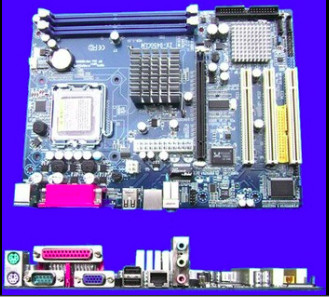
\includegraphics[width=0.700\textwidth]{./07-images/img-Ch4/Captured-Parallel-Port-Built-in-Motherboard.jpg}
				\caption{App4-Parallel Port device built-in on Motherboard (purple)}
				\label{fig:App4-Captured-Parallel-Port-Built-in-Motherboard.jpg}
			\end{center}
		 \end{figure}
		 
		
		\begin{figure}[htbp]
			\begin{center}
\frame{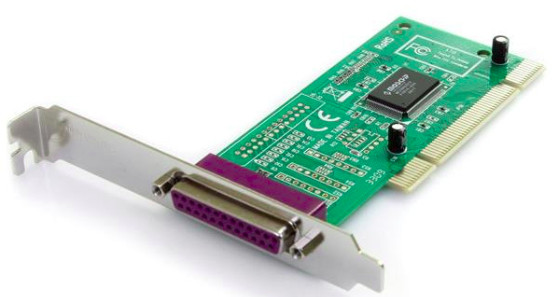
\includegraphics[width=0.65\textwidth]{./07-images/img-Ch4/Captured-Parallel-Port-PCI-Adapter-Card.jpg}}
				\caption{App4-Parallel Port PCI Adapter Card}
				\label{fig:App4-Captured-Parallel-Port-PCI-Adapter-Card.jpg}
			\end{center}
		\end{figure}
The Netmos Nm9805 is a IEEE 1284 parallel port controller with PCI bus interface. Nm9805 fully supports the existing Centronics printer interface as well as PS/2, EPP, and ECP modes. Single 5V operation. Low power. PCI compatible 1284 printer port. Multi-mode compatible controller (SPP, PS2, EPP, ECP). Fast data rates up to 1.5 Mbytes/s (parallel port). Microsoft and Linux compatible. 

% ==================
\clearpage
\pagebreak
		\begin{figure}[htbp]
			\begin{center}
\frame{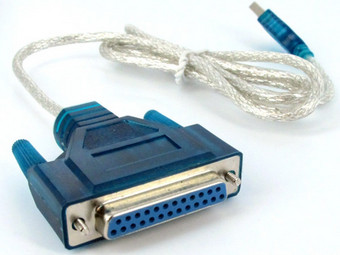
\includegraphics[width=0.65\textwidth]{./07-images/img-Ch4/Captured-USB-to-Parallel-Port-PL2305-Converter.jpg}}
				\caption{App4-USB to Parallel Port PL2305 Converter Cable}
				\label{fig:App4-Captured-USB-to-Parallel-Port-PL2305-Converter.jpg}
			\end{center}
		\end{figure}

		\begin{figure}[htbp]
			\begin{center}
\frame{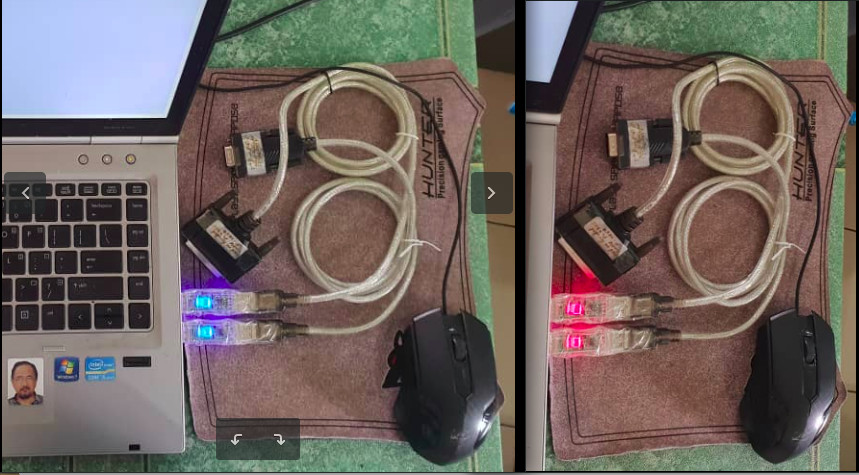
\includegraphics[width=0.75\textwidth]{./07-images/img-Ch4/USB-to-Serial-Parallel-Idle-and-Writing-Modes.jpg}}
				\caption{App4-USB to-Serial and to-Parallel Idle(Left) and Writing(Right) Modes}
				\label{fig:App4-USB-to-Serial-Parallel-Idle-and Writing-Modes.jpg}
			\end{center}
		\end{figure}
		
LEFT PICTURE: The blue color LED status is for cable device idle and ready.\\
RIGHT PICTURE: The red color LED status is for cable device busy during active reading and writing modes.  
	
\lstset{basicstyle=\ttfamily\small}
%% \lstset{basicstyle=\ttfamily\tiny}
\begin{lstlisting}[breaklines, frame=single, caption={App4-Detection of USB-to-Parallel Cable}, label=App4-usb-to-paralle-PL2305-cable-detected]
Bus 001 Device 021: ID 067b:2305 Prolific Technology, Inc. 
PL2305 Parallel Port  <=== FOUND 
[ 3978.848284] usb 1-1.6: Manufacturer: Prolific Technology Inc.
[ 3978.855271] usblp 1-1.6:1.0: usblp0: USB Bidirectional 
printer dev 21 if 0 alt 1 proto 2 vid 0x067B pid 0x2305
\end{lstlisting}

		
% ==================
\clearpage
\pagebreak
		
\subsection{App4-Velleman K8000 Parallel Interface Board}

	\begin{figure}[htbp]
		\begin{center}
\frame{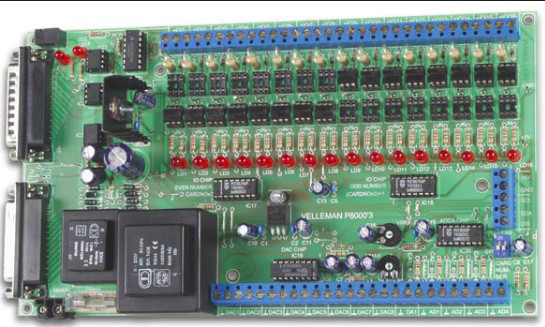
\includegraphics[width=0.85\textwidth]{./07-images/img-Ch4/Captured-Velleman-K8000-Parallel-Port-Extension-Board.jpg}}
			\caption{App4-Velleman K8000 Parallel Port Extension Board}
			\label{fig:App4-Captured-Velleman-K8000 Parallel-Port-Extension-Board.jpg}
		\end{center}
	\end{figure}
	
\lstset{basicstyle=\ttfamily\small}
%% \lstset{basicstyle=\ttfamily\tiny}
\begin{lstlisting}[breaklines, frame=single, caption={App4-Specifications of Velleman K8000 Parallel Interface Board}, label=App4-Specifications-Velleman-K8000-Interface-Board]
DIGITAL OUTPUTS:
    optocoupler, open collector output: 50mA - max. 30VDC
DIGITAL INPUTS:
    optocoupler input: 5V/5mA, max. 20V/40mA
ANALOG OUTPUTS:
    8 outputs DAC1 to DAC8, resolution: 64 steps
    minimum output voltage: 0.1V at 2mA
    maximum output voltage: 11.5V adjustable at 2mA
    resolution per step from 0.1 to 11.5V: 160mV +/- 90mV
    1 precision output DA1, resolution: 256 steps
    minimum output voltage: 0V
    maximum output voltage: 4.5V adjustable at 0.5mA
    resolution per step from 0 to 4.5V: 17.5mV
ANALOG INPUTS:
    4 analogue inputs AD1 to AD4, resolution: 256 steps
    minimum input voltage: 0V
    maximum input voltage: 5V
    input impedance: 50Mohm
    resolution: 19.5mV
    communication protocol: I2Cbus
    LED indication for each I/O
BOARD:
    25 pin D series connector for computer
    25 pin D series connector for printer
    supply voltage: 230Vac
    PCB dimensions: 237 x 133mm (9.3" x 5.2")
\end{lstlisting}			
			
%================================================		
\clearpage
\pagebreak		
		
\subsection{App4-Velleman K8055 USB Interface Board}
	
\begin{figure}[htbp]
	\begin{center}
\frame{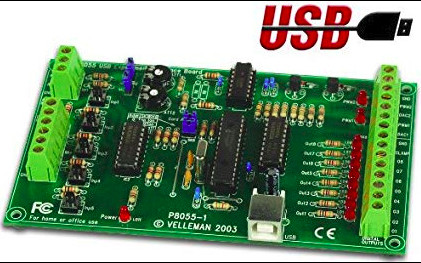
\includegraphics[width=0.85\textwidth]{./07-images/img-Ch4/Captured-Velleman-K8055-USB-Extension-Board.jpg}}
\caption{App4-Velleman K8055 USB Port Extension Board}
\label{fig:App4-Captured-Velleman-K8055-USB-Extension-Board.jpg}
	\end{center}
\end{figure}

\lstset{basicstyle=\ttfamily\small}
%% \lstset{basicstyle=\ttfamily\tiny}
\begin{lstlisting}[breaklines, frame=single, caption={App4-Specifications of Velleman K8055 USB Interface Board}, label=App4-Specifications-Velleman-K8055-USB-Interface-Board]
DIGITAL INPUTS:
    5 digital inputs (0 = ground, 1 = open) 
    (on board test buttons provided)
ANALOG INPUTS:
    2 analogue inputs with attenuation and amplification 
    option (internal test +5V provided)
DIGITAL OUTPUTS:
    8 digital open collector output switches 
    (max. 50V/100mA) (on board LED indication)
ANALOG OUTPUTS:
    2 analogue outputs:
    0 to 5V, output resistance 1K5
    PWM 0 to 100% open collector outputs 
    max 100mA / 40V (on board LED indication)
    general conversion time: 20ms per command
BOARD:    
    power supply through USB: approx. 70mA
    dimensions: 145 x 88 x 20mm / 5.7 x 3 x 0.8"
\end{lstlisting}


%================================================		
\clearpage
\pagebreak

\subsection{App4-Heber X10i USB Board}.

\begin{figure}[htbp]
	\begin{center}
		\frame{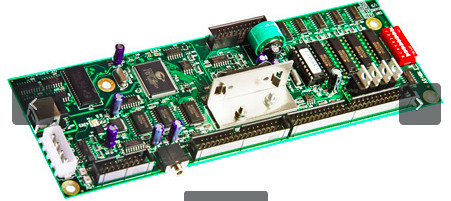
\includegraphics[width=0.85\textwidth]{./07-images/img-Ch4/Captured-Heber-X10i-USB-Extension-Board.jpg}}
		\caption{App4-Heber X10i USB Port Extension Board}
		\label{fig:App4-Captured-Heber-X10i-USB-Extension-Board.jpg}
	\end{center}
\end{figure}


\lstset{basicstyle=\ttfamily\small}
%% \lstset{basicstyle=\ttfamily\tiny}
\begin{lstlisting}[breaklines, frame=single, caption={App4-Specifications of Heber-X10i USB Interface Board}, label=App4-Specifications-Heber-X10i-USB-Interface-Board]
Heber X10i = USB real-time PC I/O controller
HARDWARE:
	64 Switched Inputs / Outputs
	Real-time I/O processor
	Battery backed SRAM
	Secure data retention
	DALLAS unique identifier
	Audio amp 5W RMS, Stereo audio amplifier
	Serial I/O
	SEC meter
	ccTalk
	LED control
	EEPROM 32KB
	Real time clock
	Current sensing 12v supply
	Open drain outputs for lamps and meters
	High current outputs
SOFTWARE:
	Serial I/O: RS232, TTL, ccTalk
	On-board security device
	Program in C, C+, C# or BlitzMax
	Microsoft Windows XPe / Linux / Raspberry Pi drivers
\end{lstlisting}

%================================================		
\clearpage
\pagebreak		
		
\subsection{App4-Arduino Due USB Board}. 

\begin{figure}[htbp]
	\begin{center}
		\frame{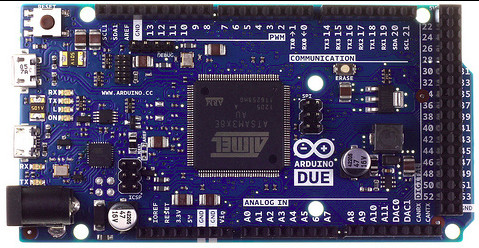
\includegraphics[width=0.85\textwidth]{./07-images/img-Ch4/Captured-Arduino-Due-USB-Extension-Board.jpg}}
		\caption{App4-Arduino Due USB Port Extension Board}
		\label{fig:App4-Captured-Arduino-Due-USB-Extension-Board.jpg}
	\end{center}
\end{figure}

Unlike most Arduino boards, the Arduino Due board runs at 3.3V. The maximum voltage that the I/O pins can tolerate is 3.3V. Applying voltages higher than 3.3V to any I/O pin could damage the board. 
\vspace*{1\baselineskip}

The SAM3X provides one hardware UART and three hardware USARTs for TTL (3.3V) serial communication.

\lstset{basicstyle=\ttfamily\small}
%% \lstset{basicstyle=\ttfamily\tiny}
\begin{lstlisting}[breaklines, frame=single, caption={App4-Specifications of Arduino Due USB Interface Board}, label=App4-Specifications-Arduino-Due-USB-Interface-Board]
Microcontroller 	AT91SAM3X8E
Operating Voltage 	3.3V
Input Voltage (recommended) 7-12V
Input Voltage (limits) 	6-16V
Digital I/O Pins 	54 (of which 12 provide PWM output)
Analog Input Pins 	12
Analog Output Pins 	2 (DAC)
Total DC Output Current on all I/O lines 	130 mA
DC Current for 3.3V Pin 	800 mA
DC Current for 5V Pin 	800 mA
Flash Memory 	512 KB all available for the user applications
SRAM 	96 KB (two banks: 64KB and 32KB)
Clock Speed 	84 MHz
Length 	101.52 mm
Width 	53.3 mm
Weight 	36 g
\end{lstlisting}

%================================================		
\clearpage
\pagebreak
		
\subsection{App4-Nexys-3 Spartan-6 FPGA USB Board}. 


\begin{figure}[htbp]
	\begin{center}
\frame{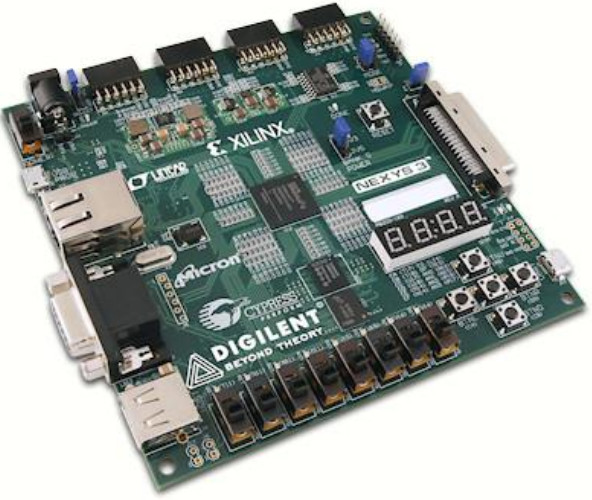
\includegraphics[width=0.80\textwidth]{./07-images/img-Ch4/Captured-Nexys3-Spartan6-FPGA-USB-Extension-Board.jpg}}
		\caption{App4-Nexys-3 Spartan-6 FPGA USB Port Extension Board}
		\label{fig:App4-Captured-Nexys3-Spartan6-FPGA-USB-Extension-Board.jpg}
	\end{center}
\end{figure}

Nexys 3 is compatible with all Xilinx CAD tools, including ChipScope, EDK, and the free WebPack. The Nexys 3 uses Digilent's newest Adept USB2 system that offers FPGA and ROM programming, automated board tests, virtual I/O, and simplified user data transfer facilities. In our project we used the Adept USB2 system.

\lstset{basicstyle=\ttfamily\small}
%% \lstset{basicstyle=\ttfamily\tiny}
\begin{lstlisting}[breaklines, frame=single, caption={App4-Specifications of Nexys-3 Spartan-6 FPGA USB Interface Board}, label=App4-Specifications-Nexys-3-Spartan-6-FPGA-USB-Interface-Board]
Xilinx Spartan-6 LX16 FPGA in a 324 pin BGA package
16 Mbyte Cellular RAM (x16)
16Mbytes SPI (quad mode) PCM non volatile memory
16Mbytes parallel PCM non volatile memory
10/100 Ethernet PHY
On board USB2 port for programming and data xfer
USB UART and USB
HID port (for mouse/keyboard)
8 bit VGA port
100 MHz CMOS oscillator
72 I/Os routed to expansion connectors
GPIO includes 8 LEDs, 5 buttons, 8 slide switches and 
4-digit seven segment display
USB v2 - programming cable included
\end{lstlisting}


%================================================		
\clearpage
\pagebreak

\subsection{App4-Raspberry Pi-3 Model-B Single Board Computer}. 

\begin{figure}[htbp]
	\begin{center}
		\frame{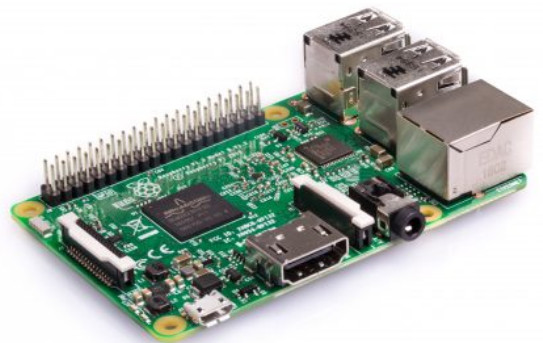
\includegraphics[width=0.85\textwidth]{./07-images/img-Ch4/Captured-Raspberry-Pi3-ModelB-SBC.jpg}}
		\caption{App4-Raspberry Pi-3 Model-B Single Board Computer}
		\label{fig:App4-Captured-Raspberry-Pi3-ModelB-SBC.jpg}
	\end{center}
\end{figure}

\subsection{App4-Raspberry Pi-2 Model-B Single Board Computer}.

\begin{figure}[htbp]
	\begin{center}
		\frame{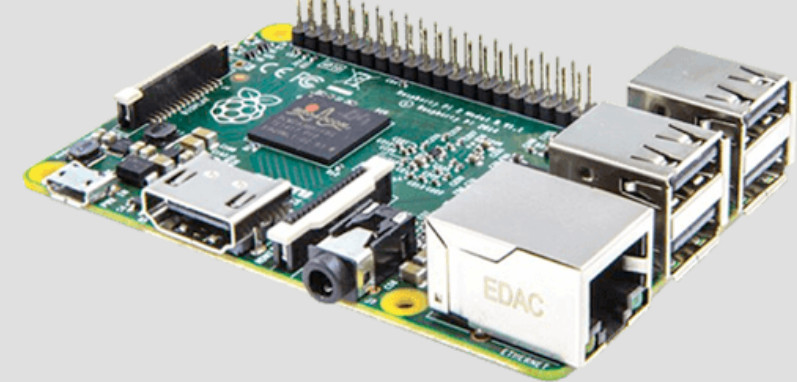
\includegraphics[width=0.85\textwidth]{./07-images/img-Ch4/Captured-Raspberry-Pi2-ModelB-SBC.jpg}}
		\caption{App4-Raspberry Pi-2 Model-B Single Board Computer}
		\label{fig:App4-Captured-Raspberry-Pi2-ModelB-SBC.jpg}
	\end{center}
\end{figure}

%================================================		
\clearpage
\pagebreak

\lstset{basicstyle=\ttfamily\small}
%% \lstset{basicstyle=\ttfamily\tiny}
\begin{lstlisting}[breaklines, frame=single, caption={App4-Specifications of Raspberry Pi 3 SBC Board}, label=App4-Specifications-of -Raspberry-Pi-3-SBC-Board]
SoC: Broadcom BCM2837
CPU: 4 x ARM Cortex-A53, 1.2GHz
GPU: Broadcom VideoCore IV
RAM: 1GB LPDDR2 (900 MHz)
Networking: 10/100 Ethernet, 2.4GHz 802.11n wireless
Bluetooth: Bluetooth 4.1 Classic, Bluetooth Low Energy
Storage: microSD
GPIO: 40-pin header, populated
Ports: HDMI, 3.5mm analogue audio-video jack, 
4 x USB 2.0, Ethernet, Camera Serial Interface (CSI), 
Display Serial Interface (DSI)
And more ....
\end{lstlisting}

\lstset{basicstyle=\ttfamily\small}
%% \lstset{basicstyle=\ttfamily\tiny}
\begin{lstlisting}[breaklines, frame=single, caption={App4-Specifications of Raspberry Pi 2 SBC Board}, label=App4-Specifications-of -Raspberry-Pi-2-SBC-Board]
SoC: Broadcom BCM2836 (CPU, GPU, DSP, SDRAM)
CPU: 900 MHz quad-core ARM Cortex A7 (ARMv7 instruction set)
GPU: Broadcom VideoCore IV @ 250 MHz
More GPU info: OpenGL ES 2.0 (24 GFLOPS); 1080p30 MPEG-2 
and VC-1 decoder (with license), h.264/MPEG-4 AVC 
high-profile decoder and encoder
Memory: 1 GB (shared with GPU)
USB ports: 4
Video input: 15-pin MIPI camera interface (CSI) connector
Video outputs: HDMI, composite video (PAL and NTSC)
via 3.5 mm jack
Audio input: I2S
Audio outputs: Analog via 3.5 mm jack; digital 
via HDMI and I2S
Storage: MicroSD
Network: 10/100Mbps Ethernet
Peripherals: 17 GPIO plus specific functions, and HAT ID bus
Power rating: 800 mA (4.0 W)
Power source: 5 V via MicroUSB or GPIO header
Size: 85.60mm x 56.5mm
Weight: 45g (1.6 oz)
\end{lstlisting}


%================================================		
\clearpage
\pagebreak

\subsection{App4-Banana Pi M2U Single Board Computer}.

\begin{figure}[htbp]
	\begin{center}
		\frame{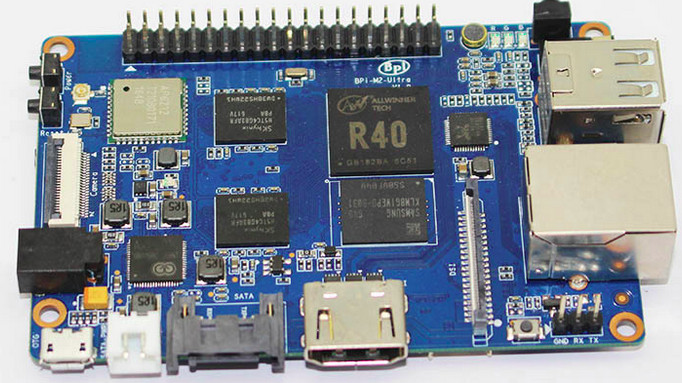
\includegraphics[width=0.85\textwidth]{./07-images/img-Ch4/Banana-PI-M2U-SBC.jpg}}
		\caption{App4-Banana Pi M2U Single Board Computer}
		\label{fig:App4-Banana-PI-M2U-SBC.jpg}
	\end{center}
\end{figure}

\lstset{basicstyle=\ttfamily\small}
%% \lstset{basicstyle=\ttfamily\tiny}
\begin{lstlisting}[breaklines, frame=single, caption={App4-Specifications of Banana Pi M2U SBC Board}, label=App4-Specifications-of -Banana-Pi-M2U-SBC-Board]
Soc 	Allwinner R40/V40
CPU 	quad-core cortex-A7,the most power efficient CPU core 
GPU 	dual-core MALI-400 MP2 and runs at 500MHz, 
GPU provides OpenGL ES 2.0, hardware-accelerated OpenVG, 
1080p45 H.264 high-profile encode and decode.
SDRAM 	2 GB DDR3 with 733MHz\(shared with GPU\)
SATA 	suppoort SATA interface
GPIO 40 Pins Header, 28 x GPIO, for UART, I2C, SPI, PWM, I2S.
On board Network 10/100/1000Mbps Ethernet\(Realtek RTL8211E)
Wifi Module 	WiFi 802.11 b/g/n \(AP 6212 module on board\)
Bluetooth 	BT4.0, Storage MicroSD\(TF\) card, 8GB eMMC 
Display 4-lane MIPI DSI display,or RGB panel, LVDS panel,
Video 	Multi-format FHD video decoding, including Mpeg1/2, 
Mpeg4, H.263, H.264, etc H.264 decode up to 1080P60,support 
Audio outputs 	HDMI, analog audio \(via 3.5 mm TRRS jack\)
Camera 	A CSI input connector Camera:Supports 8-bit YUV422 
CMOS sensor interface,Supports CCIR656 protocol for NTSC, PAL,
Supports 5M pixel camera sensor,Supports video capture 
solution up to 1080p at 30fps
Audio 	input On board microphone
USB 	2 USB 2.0 host, 1 USB 2.0 OTG
Buttons Reset button, Power button, U-boot button
Leds 	Power status Led and RJ45 Led
IR	onboard IR receiver
DC Power 5V/2A with micro USB port
battery	3.7V lithium battery power support
Sizes	85mmX56mm,same size as raspberry pi 3, Weight 40g 
\end{lstlisting}

%================================================		
\clearpage
\pagebreak

\subsection{App4-Beagle-Board xM Single Board Computer}.

\begin{figure}[htbp]
	\begin{center}
		\frame{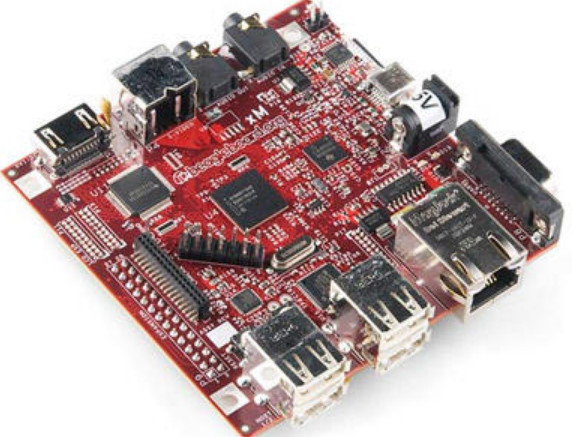
\includegraphics[width=0.85\textwidth]{./07-images/img-Ch4/Beagle-Board-xM-SBC.jpg}}
		\caption{App4-Beagle-Board xM Single Board Computer}
		\label{fig:App4-Beagle-Board-xM-SBC.jpg}
	\end{center}
\end{figure}

\lstset{basicstyle=\ttfamily\small}
%% \lstset{basicstyle=\ttfamily\tiny}
\begin{lstlisting}[breaklines, frame=single, caption={App4-Specifications of Beagle Board xM SBC Board}, label=App4-Specifications-of-Beagle-Board-xM-SBC-Board]
    Processor TI DM3730 Processor 1 GHz ARM Cortex-A8 core
    HD capable TMS320C64x+ core (800 MHz - 720p 30 fps)
    Imagination Technologies PowerVR SGX 2D/3D 
    graphics processor supporting dual independent displays
    512 MB LPDDR RAM, MicroSD/MMC card
    4 GB microSD card supplied with the BeagleBoard-xM 
    and loaded with The Angstrom Distribution
    DVI-D (HDMI connector chosen for size - maximum 
    resolution is 1400x1050)  S-Video
    USB OTG (mini AB), 4 USB ports, Ethernet
    Stereo in and out jacks
    RS-232 port  JTAG connector
    Power socket (5 V barrel connector type)
    Camera port, Expansion port
    Boot code stored on the uSD card, Boot from uSD/MMC only
    Alternative Boot source button.
    Has been demonstrated using Android,[18] 
    Angstrom Linux,[19] Fedora, Ubuntu, Gentoo,
    Arch Linux ARM and Maemo Linux distributions,
    FreeBSD, the Windows CE operating system, and RISC OS.
\end{lstlisting}

%% ===============================================